\documentclass{article}
\usepackage[paperwidth=16in,paperheight=9in,margin=0in]{geometry}
\pagestyle{empty}
\usepackage[T1]{fontenc}
\usepackage[scaled=0.92]{helvet}
\renewcommand{\familydefault}{\sfdefault}
\usepackage{xcolor}
\usepackage{tikz}
\usetikzlibrary{arrows.meta,calc,fit,backgrounds}

\definecolor{defensenavy}{HTML}{0C171F}
\definecolor{defensegreen}{HTML}{00F700}
\definecolor{datafill}{HTML}{F3F6FA}
\definecolor{constructfill}{HTML}{EEF8FA}
\definecolor{learnfill}{HTML}{F2FAF1}
\definecolor{selectfill}{HTML}{F7F2F8}
\definecolor{evalfill}{HTML}{F5F5F5}

\begin{document}
\noindent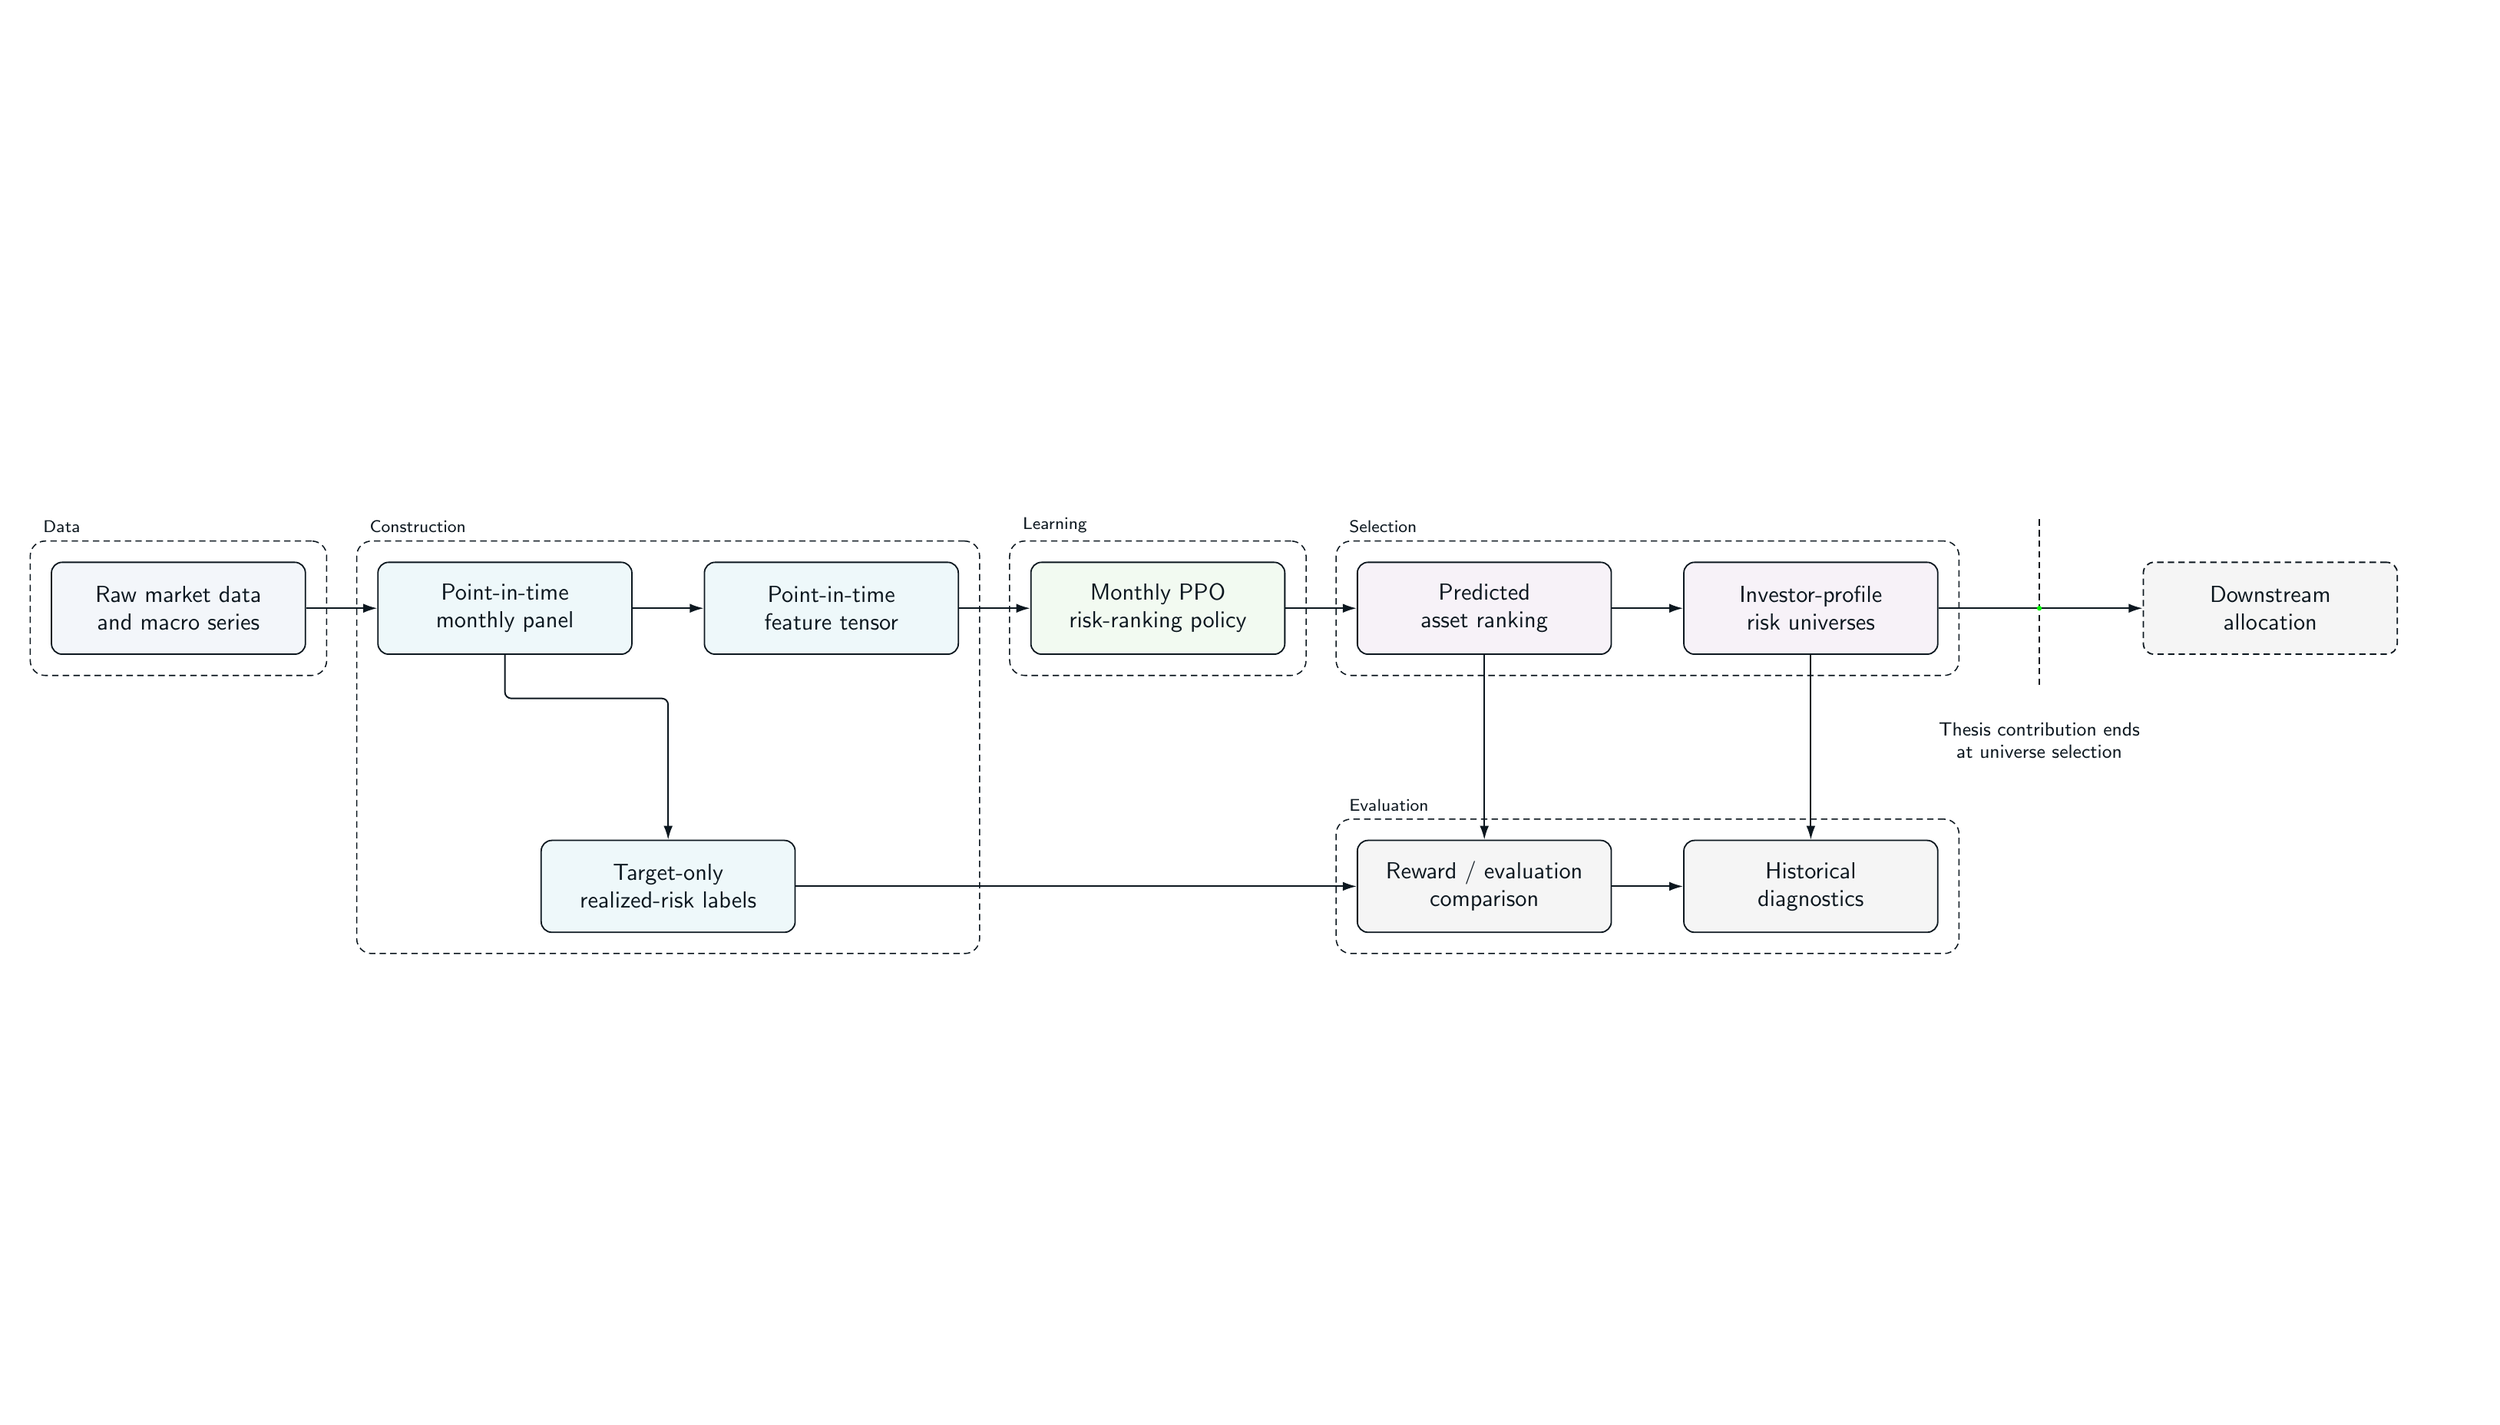
\begin{tikzpicture}[x=1cm,y=1cm,
  text=defensenavy,
  nodebox/.style={draw=defensenavy,line width=0.65pt,rounded corners=5pt,minimum width=4.2cm,minimum height=1.52cm,text width=3.72cm,align=center,inner xsep=0.20cm,inner ysep=0.18cm,font=\fontsize{11}{13}\selectfont},
  datanode/.style={nodebox,fill=datafill},
  constructnode/.style={nodebox,fill=constructfill},
  learnnode/.style={nodebox,fill=learnfill},
  selectnode/.style={nodebox,fill=selectfill},
  evalnode/.style={nodebox,fill=evalfill},
  externalnode/.style={nodebox,fill=evalfill,densely dashed},
  phase/.style={draw=defensenavy,line width=0.55pt,rounded corners=7pt,densely dashed,inner sep=0.34cm},
  phaselabel/.style={font=\fontsize{8.5}{10}\selectfont,inner xsep=0.04cm,inner ysep=0.02cm,anchor=south west},
  connector/.style={-{Latex[length=2.3mm,width=1.5mm]},draw=defensenavy,line width=0.70pt,rounded corners=3pt}
]
\path[use as bounding box] (0,0) rectangle (40.64,22.86);

% Primary process row
\node[datanode] (raw) at (2.60,13.15) {Raw market data\\and macro series};
\node[constructnode] (panel) at (8.00,13.15) {Point-in-time\\monthly panel};
\node[constructnode] (features) at (13.40,13.15) {Point-in-time\\feature tensor};
\node[learnnode] (ppo) at (18.80,13.15) {Monthly PPO\\risk-ranking policy};
\node[selectnode] (rank) at (24.20,13.15) {Predicted\\asset ranking};
\node[selectnode] (universes) at (29.60,13.15) {Investor-profile\\risk universes};
\node[externalnode] (allocation) at (37.20,13.15) {Downstream\\allocation};

% Supporting evaluation row
\node[constructnode] (target) at (10.70,8.55) {Target-only\\realized-risk labels};
\node[evalnode] (comparison) at (24.20,8.55) {Reward / evaluation\\comparison};
\node[evalnode] (diagnostics) at (29.60,8.55) {Historical\\diagnostics};

% Phase containers, drawn behind the flow
\begin{scope}[on background layer]
\node[phase,fit=(raw)] (gdata) {};
\node[phase,fit=(panel)(features)(target)] (gconstruction) {};
\node[phase,fit=(ppo)] (glearning) {};
\node[phase,fit=(rank)(universes)] (gselection) {};
\node[phase,fit=(comparison)(diagnostics)] (gevaluation) {};
\end{scope}

% Consistently offset phase labels
\node[phaselabel] at ($(gdata.north west)+(0.18,0.10)$) {Data};
\node[phaselabel] at ($(gconstruction.north west)+(0.18,0.10)$) {Construction};
\node[phaselabel] at ($(glearning.north west)+(0.18,0.10)$) {Learning};
\node[phaselabel] at ($(gselection.north west)+(0.18,0.10)$) {Selection};
\node[phaselabel] at ($(gevaluation.north west)+(0.18,0.10)$) {Evaluation};

% Primary flow
\draw[connector] (raw.east) -- (panel.west);
\draw[connector] (panel.east) -- (features.west);
\draw[connector] (features.east) -- (ppo.west);
\draw[connector] (ppo.east) -- (rank.west);
\draw[connector] (rank.east) -- (universes.west);
\draw[connector] (universes.east) -- (allocation.west);

% Supporting flow; orthogonal routes keep connectors away from labels
\draw[connector] (panel.south) -- ++(0,-0.72) -| (target.north);
\draw[connector] (target.east) -- (comparison.west);
\draw[connector] (rank.south) -- (comparison.north);
\draw[connector] (comparison.east) -- (diagnostics.west);
\draw[connector] (universes.south) -- (diagnostics.north);

% Explicit thesis-to-downstream handoff
\draw[defensenavy,densely dashed,line width=0.60pt] (33.38,14.62) -- (33.38,11.82);
\fill[defensegreen] (33.38,13.15) circle (1.15pt);
\node[align=center,font=\fontsize{9}{10.5}\selectfont,text=defensenavy]
  at (33.38,10.96) {Thesis contribution ends\\at universe selection};

\end{tikzpicture}
\end{document}
